% Source-derived chapter 03: The degeneration and dimension bounds
% Original source: refined-brill-noether-theory-hurwitz-spaces
\chapter{The degeneration and dimension bounds}
\label{refined-brill-noether-theory-hurwitz-spaces-chapter-03}
\source{refined-brill-noether-theory-hurwitz-spaces}

\begin{remark}[Source section]
\label{refined-brill-noether-theory-hurwitz-spaces-chapter-03-source}
\source{refined-brill-noether-theory-hurwitz-spaces}
\source{refined-brill-noether-theory-hurwitz-spaces}
This chapter reproduces the corresponding section of the retrieved
LaTeX source, including its definitions, statements, examples, and
proofs. It has not yet been translated into Lean.
\notready
\end{remark}

% The source section title was: The degeneration and dimension bounds
\label{dimbounds}
\source{refined-brill-noether-theory-hurwitz-spaces}
In this section, we describe our degeneration to a chain of elliptic curves and prove a smoothing theorem for endomorphisms of the push forwards of line bundles. This involves explicit compatibility conditions at the nodes, in a manner similar to Eisenbud-Harris' proof of the Brill-Noether theorem \cite{EH} (see also \cite[Ch. 5]{HM} for an exposition). A noteworthy difference in the set up is that elliptic curves in the middle of our chain have more than one node, creating subtleties in how these conditions interact.
Also, instead of tracking vanishing sequences of different limit line bundles, we describe the sections that smooth from a fixed limit.

 
 A consequence of our analysis will be that
\begin{equation} \label{equiv}
\source{refined-brill-noether-theory-hurwitz-spaces}
\dim\{L \in \Pic^d(C) : h^0(\pp^1, End(f_*L)) \geq \delta+k^2\} \leq g - \delta.
\end{equation}
for all $\delta \geq 0$. 
Since $End(f_*L)$ is rank $k^2$ and degree $0$ on $\pp^1$,
\[u(f_*L) = h^1(\pp^1, End(f_*L)) =  h^0(\pp^1, End(f_*L)) - k^2,\]
so \eqref{equiv} implies $\dim \Sigma_{\vec{e}}(C, f) \leq g - u(\vec{e})$ for all $\vec{e}$.
(Notice that \eqref{equiv} does not refer to a particular splitting type!)

Basic cohomological observations determine all push forwards of line bundles from elliptic curves.
\begin{Lemma}
\source{refined-brill-noether-theory-hurwitz-spaces}
\notready \label{ezpush}
\source{refined-brill-noether-theory-hurwitz-spaces}
Let $X$ be an elliptic curve and $f\colon  X \rightarrow \pp^1$ a degree $k$ map. Let $L$ be a line bundle of degree $d = a + nk$ on $X$ with $0 \leq a < k$. We have
\[f_*L = \begin{cases}  \O_{\pp^1}(n-2) \oplus \O_{\pp^1}(n-1)^{\oplus k-2} \oplus  \O_{\pp^1}(n) &\text{if $L = f^*\O_{\pp^1}(n)$} \\  \O_{\pp^1}(n-1)^{\oplus k-a} \oplus \O_{\pp^1}(n)^{\oplus a} &\text{otherwise.} \end{cases}\]
 \end{Lemma}
\begin{proof}
Let $H = f^*\O_{\pp^1}(1)$. By the projection formula, $f_* L = \O_{\pp^1}(n) \otimes f_* L(-nH)$, so it suffices to consider the case $n = 0$.
First observe that $h^0(X,\O_X) = h^1(X,\O_X) = 1$. The only rank $k$ vector bundle on $\pp^1$ with this cohomology is $\O_{\pp^1}(-2) \oplus \O_{\pp^1}(-1)^{\oplus k-2} \oplus \O_{\pp^1}$ so this must be $f_*\O_X$, completing the first case.
Now suppose $L$ is non-trivial of degree $0 \leq a < k$. By Serre duality, $h^1(X,L) = h^0(X,L^\vee) = 0$, implying all summands of $f_*L$ are degree at least $-1$. Riemann-Roch shows $h^0(X,L) = a$ and moreover, $h^0(X,L(-H)) = 0$, because in this case $\deg L(-H) < 0$. It follows that $f_*L = \O(-1)^{\oplus k-a} \oplus \O_{\pp^1}^{\oplus a}$, completing the second case.
\end{proof} 




We now describe our degeneration. Let $\X_0$ be a simply nodal chain of elliptic curves $X_1, \ldots, X_g$ with $X_i$ joined to $X_{i+1}$ at a point $p_i$.
For each $i$, let $f_i: X_i \rightarrow \pp^1$ be a degree $k$ map that is totally ramified at $p_{i-1}$ and $p_i$. 
Note then that $p_{i-1}$ and $p_{i}$ differ by a $k$-torsion element on $X_i$.
Together, the $f_i$ define a map of $\X_0$ to a simply nodal chain $\P_0$ of $\pp^1$'s, labeled $P_1, \ldots, P_g$, with nodes $f_i(p_i) = f_{i+1}(p_i)$ for $1 \leq i \leq g-1$.

\vspace{.15in}
\begin{center}
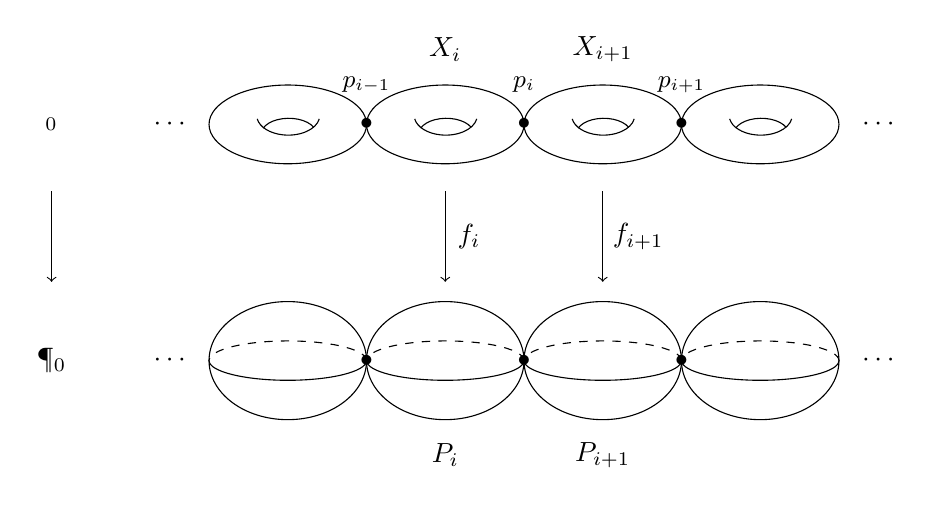
\begin{tikzpicture}
\draw (0,0) ellipse (1cm and .5cm);
 \draw (.4,.07) arc(-10:-170:.4cm and .25cm);
 \draw (.33,-.038) arc(25:158:.35cm and .2 cm);
\draw (-1, 0) node {\small $\bullet$};
\draw (1, .5) node {\small $p_{i+1}$};
\draw (-1, .5) node {\small $p_i$};
\draw (-3, .5) node {\small $p_{i-1}$};
\draw (-7, 0) node {$\X_0$};
\draw (-7, -3) node {$\P_0$};
\draw [->] (-7, -.85) -- (-7, -2);
%\draw (-7-.2, -1 -.425) node {$\f$};
\draw (-2, .95) node{$X_i$};
\draw (0, .95) node{$X_{i+1}$};
\draw [->] (-2, -.85) -- (-2, -2);
\draw (-1.7, -1 -.425) node {$f_i$};
\draw [->] (-2+2, -.85) -- (-2+2, -2);
\draw (-1.7+2.15, -1 -.425) node {$f_{i+1}$};
\draw (-2, -4.2) node{$P_i$};
\draw (0, -4.2) node{$P_{i+1}$};
\draw (2,0) ellipse (1cm and .5cm);
 \draw (2.4,.07) arc(-10:-170:.4cm and .25cm);
 \draw (2.33,-.038) arc(25:158:.35cm and .2 cm);
\draw (1, 0) node {\small $\bullet$};
\draw (1, -3) node {\small $\bullet$};
\draw (-1, -3) node {\small $\bullet$};
\draw (-3, -3) node {\small $\bullet$};
\draw (-2,0) ellipse (1cm and .5cm);
 \draw (.4 -2,.07) arc(-10:-170:.4cm and .25cm);
 \draw (.33-2,-.038) arc(25:158:.35cm and .2 cm);
 \draw (-4,0) ellipse (1cm and .5cm);
 \draw (.4 -4,.07) arc(-10:-170:.4cm and .25cm);
 \draw (.33-4,-.038) arc(25:158:.35cm and .2 cm);
\draw (-3, 0) node {\small $\bullet$};
\draw (-5.5, 0) node {$\cdots$};
\draw (3.5, 0) node {$\cdots$};
\draw (-5.5, -3) node {$\cdots$};
\draw (3.5, -3) node {$\cdots$};
\draw (0, -3) ellipse (1cm and .75cm);
 \draw (1,-3) arc(0:-180:1cm and .25cm);
  \draw[dashed] (1,-3) arc(0:180:1cm and .25cm);
  \draw (2, -3) ellipse (1cm and .75cm);
 \draw (1+2,-3) arc(0:-180:1cm and .25cm);
  \draw[dashed] (1+2,-3) arc(0:180:1cm and .25cm);
    \draw (-2, -3) ellipse (1cm and .75cm);
 \draw (1-4,-3) arc(0:-180:1cm and .25cm);
  \draw[dashed] (1-4,-3) arc(0:180:1cm and .25cm);
   \draw (-4, -3) ellipse (1cm and .75cm);
    \draw (1-2,-3) arc(0:-180:1cm and .25cm);
  \draw[dashed] (1-2,-3) arc(0:180:1cm and .25cm);
\end{tikzpicture}
\end{center}
By the theory of admissible covers \cite{admiss}, the nodes smooth to obtain a family $\f\colon  \mathcal{X} \rightarrow \mathcal{P}$, flat over a pointed smooth curve $(\Delta, 0)$, where the general fiber is a smooth curve of genus $g$ mapping to $\pp^1$ and the central fiber is the map $\X_0 \rightarrow \P_0$ restricting to $f_i$ on each component $X_i$. (For a treatment in positive characteristic see Section 5 of \cite{liu}.)
 By slight abuse of notation, we also write $\f$ for this map on the central fiber.
 We write $\tilde{\X} \rightarrow \tilde{\P}$ for the family over the punctured curve $\Delta \backslash \{0\}$.

The curve $\X_0$ is compact type. In particular, given a degree $d$ line bundle $\tilde{\L}$ on $\tilde{\X}$ and 
 partition $d = d_1 + \ldots + d_g$, there is a unique extension $\mathcal{L}$ to $\X$ so that the limit $\L_0 = \L|_{\X_0}$ restricts to a degree $d_i$ line bundle $L_i$ on $X_i$.  We wish to bound $h^0(\P_t, End(\f_*\L_t))$ for general $t$. To do so, we study the subspace of $V_\L \subset H^0(\P_0, End(\f_*\L_0))$ of sections which arise as limits of sections in $H^0(\P_t, End(\f_*\L_t))$ as $t \rightarrow 0$.

 For simplicity, let us fix a partition $d_1 + \ldots + d_g = d$ and
 write 
 \[\Pic^d(X) := \Pic^{d_1}(X_1) \times \Pic^{d_2}(X_2) \times \cdots \times \Pic^{d_g}(X_g).\]  
 Let $\alpha_i : X_i \rightarrow \X_0$ denote the inclusion.
 Given $\L_0 = (L_1, \ldots, L_g) \in \Pic^d(\X_0)$, we have a short exact sequence on $\X_0$
 \[0 \rightarrow \L_0 \rightarrow \bigoplus_{i=1}^g (\alpha_i)_* L_i \rightarrow \bigoplus_{i=1}^{g-1} \O_{p_i} \rightarrow 0.\] 
Let $\beta_i : P_i \rightarrow \P_0$ be the inclusion.
For each $i$, let $E_i = (f_i)_* L_i$.
Applying $\f_*$ to the above, we obtain an exact sequence on $\P_0$
 \begin{equation} \label{flseq}
\source{refined-brill-noether-theory-hurwitz-spaces}
 0 \rightarrow \f_*\L_0 \rightarrow \bigoplus_{i=1}^g (\beta_i)_*E_i \rightarrow \bigoplus_{i=1}^g \O_{f(p_i)} \rightarrow 0.
 \end{equation}
\begin{warning}
The map $\f|_{\X_0}: \X_0 \rightarrow \P_0$ is not flat and $\f_*\L_0$ is \text{not} locally free at the nodes $\f(p_i)$. Nevertheless, our family is flat over the curve $\Delta$, so $\f_*\L_0 = (\f_*\L)|_{\P_0}$ is the limit we wish to consider.
\end{warning}
The restriction of $\f_*\L_0$ to each component $P_i$ has an isomorphism
\begin{equation} \label{compiso}
\source{refined-brill-noether-theory-hurwitz-spaces}
(\f_*\L_0)|_{P_i} \cong E_i \oplus \O_{\f(p_{i-1})}^{\oplus k-1} \oplus \O_{\f(p_i)}^{\oplus k-1}.
\end{equation}
In what follows, we will write $L_i|_{kp}$ for $L_i|_{f_i^{-1}(f_i(p))}$.
Above, $\O_{\f(p_{i-1})}^{\oplus k-1}$ is identified with the subspace of $H^0(L_{i-1}|_{kp_{i-1}})$ of functions vanishing at $p_{i-1}$ and 
$\O_{\f(p_{i})}^{\oplus k-1}$ is identified with the subspace of $H^0(L_{i+1}|_{kp_i})$ of functions vanishing at $p_{i}$.
The splitting of the middle term is defined by the map sending a section $\sigma$ to $\sigma|_{kp_{i-1}} - \sigma(p_{i-1}) \in H^0(L_{i-1}|_{kp_{i-1}})$. We think of the $k-1$ factors $\O_{f(p_{i-1})}^{\oplus k-1}$ as remembering the values of the first $k-1$ derivatives of $\sigma$ at $p_{i-1}$ along $X_{i-1}$, and similarly the $k-1$ factors $\O_{f(p_{i})}$ as remembering the values of the first $k-1$ derivatives of $\sigma$ at $p_{i}$ along $X_{i+1}$.

Applying $Hom(\f_*\L_0, -)$ to \eqref{flseq} and using \eqref{compiso}, we obtain an injection of sheaves
\[End(\f_*\L_0) \hookrightarrow \bigoplus_{i = 1}^g Hom(\f_*\L_0, (\beta_i)_*E_i) \cong \bigoplus_{i=1}^g Hom((\f_*\L_0)|_{P_i}, E_i) \cong \bigoplus_{i=1}^g End(E_i).\]
The last isomorphism follows because there are no non-zero maps from the torsion summands to a locally free sheaf.
Taking global sections yields an inclusion
\[ \iota: H^0(\P_0, End(\f_*\L_0)) \hookrightarrow \bigoplus_{i=1}^g H^0(P_i, End(E_i)).\]
We want to describe the image under $\iota$ of the subspace $V_\L \subset H^0(\P_0, End(\f_*\L_0))$ of sections that arise as limits from smooth curves. One necessary condition on each factor is described in the following definition. In what follows $\cc$, denotes the ground field, which is algebraically closed of any characteristic.
\begin{Definition}
\source{refined-brill-noether-theory-hurwitz-spaces}
\notready
Let $L$ be a line bundle on an elliptic curve with a degree $k$ map $f\colon  X \rightarrow \pp^1$ and let $E = f_* L$. Given a point $p$ of total ramification of $f$,
we say $\phi \in H^0(\pp^1, End(E))$ is \textit{order preserving at $p$} if $\ord_p(\phi(\sigma)) \geq \ord_p \sigma$ for all $\sigma \in H^0(U, L)$ for any $U \ni p$. Equivalently, the restriction $\res \phi \in \End(H^0(L|_{kp})) \cong \End(\cc[x]/(x^k))$ is lower triangular with respect to the basis $1, x, x^2, \ldots, x^{k-1}$. 
Note that the diagonal entries $d_{p}^{(j)}(\phi) := (\res \phi)(x^j)/x^j|_{x=0}$ are independent of choice of local coordinate $x$.
\end{Definition}

We now describe agreement conditions near the nodes that are satisfied by every element of $\iota(V_\L)$.
 \begin{Lemma}
\source{refined-brill-noether-theory-hurwitz-spaces}
\notready \label{cond}
\source{refined-brill-noether-theory-hurwitz-spaces}
Given $\L_0 = (L_1, \ldots, L_g) \in \Pic^d(\X_0)$, let $\L$ be a line bundle on $\X$ such that $\L|_{\X_0} = \L_0$.
Let $V_\L \subset H^0(\P_0, End(\f_*\L_0))$ be the subspace of sections that can be extended to $H^0(\P, End(\f_*\L))$.
If $(\phi_1, \ldots, \phi_g) \in \iota(V_\L)$ then the following conditions hold for each $i=1, \ldots, g-1$:
\begin{enumerate}
\item \label{x} $\phi_i$ is order preserving at $p_i$
\source{refined-brill-noether-theory-hurwitz-spaces}
\item \label{y} $\phi_{i+1}$ is order preserving at $p_i$
\source{refined-brill-noether-theory-hurwitz-spaces}
\item \label{d} We have $d_{p_i}^{(0)}(\phi_i) = d_{p_i}^{(0)}(\phi_{i+1})$ and $d_{p_i}^{(j)}(\phi_i) = d_{p_i}^{(k-j)}(\phi_{i+1})$ for $j = 1, \ldots, k-1$.
\source{refined-brill-noether-theory-hurwitz-spaces}
 \end{enumerate}
 \end{Lemma}
 
 \begin{proof}
 It suffices to work locally around $p_i$. 
 Let $\cc$ be the ground field, which is algebraically closed of any characteristic.
 We may choose formal local coordinates $x, y, t$ near $p_i$ so that $\widehat{\O}_{\X, p_i} = \cc\ll x, y \rr /(xy - t)$ and $\widehat{\O}_{\P, \f(p_i)} = \cc\ll a, b \rr /(ab - t^k)$ and the map $\f$ is described locally by a map $\cc\ll a, b, t \rr /(ab - t^k) \rightarrow \cc\ll x, y, t \rr/(xy - t)$ such that $a \mapsto x^k u^{-1}$ and $b \mapsto y^k u$ for $u$ a power series in $x, y$ with constant coefficient $1$. (If the characteristic of $\cc$ does not divide $k$, we can extract a $k$th root of $u$ and absorb it into $x$ and $y$, and thereby assume $u  = 1$.)
 
 Since $\L$ is locally free, a section of $End(\f_*\L)$ is given locally near $\f(p_i)$ by an an endomorphism $\psi$ of $\cc\ll x, y, t \rr/(xy - t)$ viewed as an $\cc\ll a, b, t \rr /(ab - t^k) $ module. 
On the central fiber, the monomials $1, x, x^2, \ldots, x^{k-1}, y, y^2, \ldots, y^{k-1}$ generate $\cc\ll x, y \rr/(xy)$ as a module over $\cc\ll a, b \rr /(ab)$. By Nakayama's lemma, these monomials generate $\cc\ll x, y, t \rr/(xy - t)$ as an $\cc \ll a, b, t \rr /(ab - t^k)$ module. Because $\psi$ is a module homomorphism, we have
 \begin{align}
  (y^ku) \cdot \psi(x^j) &= b \cdot \psi(x^j) = \psi(b \cdot x^j) = \psi(y^{k-j} \cdot u \cdot (y^jx^j)) \notag \\
  &= \psi(y^{k-j} \cdot u \cdot t^j) = \psi(y^{k-j} \cdot u) \cdot t^j = \psi(y^{k-j} \cdot u) \cdot x^jy^j. \label{calc}
\source{refined-brill-noether-theory-hurwitz-spaces}
  \end{align}
Hence, $x^j$ divides $\psi(x^j)$. A similar argument shows that $y^{j}$ divides $\psi(y^{j})$. Thus, $\psi$ is order-preserving, so conditions \eqref{x} and \eqref{y} are satisfied.
Moreover, since $xy = t$, we see that $x^iy^j$ divides 
\[\psi(x^i y^j) = \begin{cases} t^{i} \psi(y^{j -i})  =  x^{i} y^i \psi(y^{j -i}) & \text{if $i \leq j$} \\ t^j \psi(x^{i - j}) =  x^jy^j \psi(x^{i - j}) &\text{if $j \leq i$} \end{cases}\]
for all $i, j$. Since $u = 1 + (x, y)$, it follows that $\psi(y^{k-j} \cdot u) = \psi(y^{k-j}) + y^{k-j} \cdot (x, y)$.
Dividing both sides of $\eqref{calc}$ by $x^j y^{k}$, we see that
 \[u \cdot \frac{\psi(x^j)}{x^j} = \frac{\psi(y^{k-j} \cdot u)}{y^{k-j}} = \frac{\psi(y^{k-j})}{y^{k-j}} + (x, y).\]
When $j = 1 , \ldots, k-1$, setting $x = y = 0$ in the equation above establishes part (3). (The case $d^{(0)}_{p_i}(\phi_i) = d_{p_i}^{(0)}(\phi_{i+1})$ follows from the fact that both are equal to the constant term of $\psi(1)$.)
It follows that any collection $(\phi_1, \ldots, \phi_g)$ which arrises as a limit of a section defined on smooth curves must satisfy these local compatibility properties near the nodes.
   \end{proof}
 
 Notice that conditions \eqref{x} and \eqref{y} of Lemma \ref{cond}  each represent $k(k-1)/2$ linear conditions on $\phi_i$ and $\phi_{i+1}$. Condition \eqref{d} represents another $k$ linear conditions on $\phi_i$ and $\phi_{i+1}$, for a total of $k^2$ possible linear conditions near each node. Our next task is to show that these conditions are all independent for general $(L_1, \ldots, L_g)$, and bound the dimension of the subvarieties inside $\Pic^d(\X_0)$ where they fail to be independent by a certain amount.
 The key technical lemma is to establish when the constraints on $\phi_i \in H^0(P_i, End(E_i))$ coming from the two different nodes $p_i$ and $p_{i+1}$ are independent.
   
 \begin{Lemma}
\source{refined-brill-noether-theory-hurwitz-spaces}
\notready \label{zing}
\source{refined-brill-noether-theory-hurwitz-spaces}
Suppose we have an elliptic curve with a degree $k$ map $f\colon  X \rightarrow \pp^1$ which is totally ramified over two distinct points $p, q \in X$. Let $L$ be a line bundle on $X$ which is not isomorphic to $f^*\O_{\pp^1}(n)$ for any $n$, and set $E = f_*L$. 
 Let $W_p \subset H^0(\pp^1,End(E))$ (respectively $W_q \subset H^0(\pp^1, End(E))$) denote the subspace of sections which are order preserving at $p$ (respectively $q$).
 Then, 
 \[\dim W_q = \begin{cases} \frac{k(k+1)}{2} + 1 & \text{if $L \cong \O_X(mq)$ for some $m$} \\ \frac{k(k+1)}{2} & \text{otherwise}\end{cases}\]
 and
 \[\dim W_p \cap W_q = \begin{cases} k+1 & \text{if $L \cong \O_X(n p+ m q)$ for some $m, n$} \\ k & \text{otherwise}. \end{cases} \]
 Moreover, the map $\diag: W_p \cap W_q \rightarrow \cc^{\oplus k}$ given by
 \begin{equation} \label{map}
\source{refined-brill-noether-theory-hurwitz-spaces}
 \phi \mapsto \left(d_{p}^{(0)}(\phi), \ldots, d_{p}^{(k-1)}(\phi)\right)
 \end{equation}
 is surjective. Finally, if $\phi \in \ker(\diag) \cap W_p \cap W_q$, then $\phi$ can be represented by a matrix with at most one non-zero entry.
 \end{Lemma}
 \begin{proof}
 The rough idea is to choose a decomposition of $E$ so that the condition of being order preserving at $p$ is that a matrix for an endomorphism is lower triangular, while the condition of being order preserving at $q$ is that the matrix is upper triangular. We shall see that if $L \ncong \O_X(np + mq)$, then the conditions to be order preserving and $p$ and at $q$ are independent, while if 
 $L \cong \O_X(np + mq)$ we obtain one less condition.
Twisting $L$ by $f^*\O_{\pp^1}(1)$ does not change $End(E)$, so we assume $k \leq \deg L < 2k$.
 
We first prove the case when $L \ncong \O_X(np + mq)$. 
By Lemma \ref{ezpush}, $E \cong \O_{\pp^1}^{\oplus k-a} \oplus \O_{\pp^1}(1)^{\oplus a}$ where $a = \deg L - k$.
Let $s, t \in f^*\O_{\pp^1}(1)$ denote sections defining the map $f$ with $V(s) = kq$ and $V(t) = kp$. For each $0 \leq j \leq a-1$, and $\alpha, \beta \in \cc$, there is a section $\tau_j(\alpha, \beta)= (\alpha s + \beta t) \cdot u_j \in H^0(X, L)$
 where $V(u_j) = jp + (a-1-j)q + r_j$. Note that $r_j \neq p, q$ by assumption. For each $j$, the $\tau_j(\alpha, \beta)$ span a copy of $H^0(\pp^1, \O_{\pp^1}(1))$ inside $H^0(\pp^1, E) = H^0(X, L)$. For $a \leq j \leq k-1$, we choose $\sigma_j \in H^0(X, L)$ so that $V(\sigma_j) =  jp + (k+a-1-j)q + r_j$, where again $r_j \neq p,q$. 
These $\sigma_j$ are non-vanishing on fibers of $f$, so each corresponds to an $H^0(\pp^1, \O_{\pp^1})$ factor inside $H^0(\pp^1, E) = H^0(X, L)$.
With respect to this decomposition of $E$, an element of $H^0(\pp^1, End(E))$ is represented by a block upper triangular matrix where the two diagonal blocks consist of elements of $\cc$ and the upper block consists of linear forms.
 \begin{equation} \label{mat}
\source{refined-brill-noether-theory-hurwitz-spaces}
\phi =  \left( \begin{matrix}
 c_{0,0} & \cdots & c_{0,a-1} & \alpha_{0, a} s + \beta_{0, a} t & \cdots & \alpha_{0, k-1} s + \beta_{0, k-1}t \\
  c_{1,0} & \cdots & c_{1,a-1} & \alpha_{1, a} s + \beta_{1, a} t & \cdots & \alpha_{1, k-1} s + \beta_{1, k-1}t \\
  \vdots & \ddots & \vdots & \vdots & \ddots & \vdots \\
   c_{d-1,0} & \cdots & c_{a-1,a-1} & \alpha_{a-1, a} s + \beta_{a-1, a} t & \cdots & \alpha_{a-1, k-1} s + \beta_{a-1, a-1}t \\
   0 & \cdots & 0 & c_{a,a} & \cdots & c_{a,k-1} \\
   0 & \cdots & 0 & c_{a+1,a} & \cdots & c_{a+1,k-1} \\
     \vdots & \ddots & \vdots & \vdots & \ddots & \vdots \\
        0 & \cdots & 0 & c_{k-1,a} & \cdots & c_{k-1,k-1} \\
 \end{matrix} \right)
 \end{equation}
 For $\ell \geq a$ and $j \geq a$, the coefficients $\alpha_{\ell, j}$ and $\beta_{\ell, j}$ specify which $\tau_\ell(\alpha_{\ell, j}, \beta_{\ell, j})$ appears in the image of $\sigma_j$ with respect to our chosen decomposition of $H^0(\pp^1, E)$.
 The condition for $\phi$ to be order preserving at $p$ is that $\alpha_{\ell, j} = 0$ for all $\ell, j$ and $c_{\ell, j} = 0$ for all $\ell < j$. Hence, $\dim W_p = k(k+1)/2$. The condition for $\phi$ to be order preserving at $q$ is that $\beta_{\ell, j} = 0$ for all $\ell, j$ and $c_{\ell, j} = 0$ for all $\ell > j$. It follows that $\dim W_p \cap W_q = k$ and, as the diagonal entries are unconstrained, $\diag$ is a surjection. Hence, $\ker(\diag) \cap W_p \cap W_q = \{0\}$.


Now suppose $L \cong \O_X(n p + mq) \ncong \O_X(kp)$. Without loss of generality, we may assume that $n \geq m > 0$. Since $n + m = a+ k$ with $a < k$, we also have $n > a$. Again, we have $E \cong \O_{\pp^1}^{\oplus k-a} \oplus \O_{\pp^1}(1)^{\oplus a}$, but the argument in the previous paragraph must be modified because $r_{n-1} = p$ and $r_n = q$ (or when $n = k$, we have $r_{k-1} = p$ and $r_0 = q$). Instead, for $a \leq j \leq k-1$, we choose $\sigma_j \in H^0(\pp^1, E)$ so that $\ord_p(\sigma_j) = j$ and
\[\ord_{q}(\sigma_j) = \begin{cases} k+a-n & \text{if $j = n$} \\ k + a - n - 1&\text{if $j = n-1$} \\  k+a - j - 1 & \text{otherwise.} \end{cases}\]
If $n = k$, then the first case above never occurs, but we must take $\tau_0(\alpha, \beta) = (\alpha s + \beta t) \cdot u_0$ where $V(u_0) = aq$.
Otherwise, the vanishing orders of $\tau_j$ and $u_j$ may be taken as before.

If $n \neq k$, then 
the condition for $\phi$ in \eqref{mat} to be order preserving at $p$ is that $\alpha_{\ell, j} = 0$ for all $\ell, j$ and $c_{\ell, j} = 0$ for all $\ell < j$. The condition for $\phi$ to be order preserving at $q$ is that all $\beta_{\ell, j} = 0$; and $c_{\ell,j} = 0$ for all $\ell > j$ with $(\ell, j) \neq (n, n-1)$; and $c_{n-1,n} = 0$. Note that $c_{n,n-1}$ need not vanish because $\ord_q(\sigma_{n}) > \ord_q(\sigma_{n-1})$. 

In the case $n=k$, the condition for $\phi$ to be order preserving at $q$ is that $c_{\ell,j} = 0$ for all $\ell > j$  and $\beta_{\ell, j} = 0$ for all $(\ell, j) \neq (0, k-1)$. Note that $\beta_{0, k-1}$ is not required to vanish because $\ord_q(\sigma_{k-1}) = a-1 < a = \ord_q(u_0)$ so $\beta_{0, k-1}$ is not required to vanish. Thus, $\dim W_q =\frac{k(k+1)}{2}+1$. Note that $n = k$ corresponds to the case when $L \cong \O((n+m)q)$.
Our explicit description shows that $\dim W_p \cap W_q = k+1$, and the intersection consists of matrices with arbitrary diagonal entries and at most one non-zero off-diagonal entry. Hence, in all cases, $\ker(\diag) \cap W_p \cap W_q$ consists of matrices with at most one non-zero entry.
   \end{proof}

Having characterized necessary compatibility conditions at the nodes and when they are independent,
we now prove \eqref{equiv}. This will be subsumed by the results of the next section, but we include it here as the proof indicates subvarieties of $\Pic^d(\X_0)$ where the limits of line bundles with a certain splitting type must live.

\begin{Lemma}
\source{refined-brill-noether-theory-hurwitz-spaces}
\notready \label{dimbound}
\source{refined-brill-noether-theory-hurwitz-spaces}
Let $f\colon  C \rightarrow \pp^1$ be a general genus $g$, degree $k$ cover. Then
\[\dim \Sigma_{\vec{e}}(C, f) \leq g - u(\vec{e}).\]
\end{Lemma}
\begin{proof}
The case $g = 1$ was proved in Lemma \ref{ezpush}, so we assume $g > 1$. Since we are also assuming $k > 2$, we can choose a degree distribution $d = d_1 + \ldots + d_g$ so that no $d_i$ is a multiple of $k$. In particular, given $\L_0 = (L_1, \ldots, L_g) \in \Pic^d(\X_0)$, we may assume that $L_i \ncong f^*\O(n)$.
Define
\[\epsilon_i = \begin{cases} 1 & \text{if $i \neq 1, g$ and $L_i \cong  \O_{X_i}(np_{i-1} + mp_i)$} \\ 1 & \text{if $i = 1$ and $L_1 \cong \O_{X_1}(mp_1)$} \\ 1 & \text{if $i = g$ and $L_g \cong \O_{X_g}(np_{g-1})$} \\ 0 &\text{otherwise.} \end{cases}\]
By Lemmas \ref{cond} and \ref{zing},
\begin{align*}
\dim V_{\L} &\leq \sum_{i=1}^g \dim \{\phi \in H^0(P_i, End(E_i)) : \phi \text{ order preserving at nodes on $X_i$}\} - k(g-1) \\
&\leq \frac{k(k+1)}{2} +\epsilon_1 + \frac{k(k+1)}{2} +\epsilon_g + \sum_{i=2}^{g-1} (k + \epsilon_i ) - k(g-1)\\
&\leq k^2 + \delta
\end{align*}
where $\delta$ is the number of $i$ for which $L_i \cong \O_{X_i}(np_{i-1} + mp_{i})$ for some $m, n$ (with $m = 0$ if $i = 1$ and $n = 0$ if $i = g$).  In particular, the codimension of the subvariety of line bundles $\L_0$ in $\Pic^d(X)$ for which $V_{\L} \geq k^2 + \delta$ is at least $\delta$. This implies that for general $\f_t: \X_t \rightarrow \P_t$ in the family $\f\colon  \X \rightarrow \P$, 
\[\dim\{L \in \Pic^d(\X_t) : h^0(\P_t, End((\f_t)_*L)) \geq \delta +k^2\} \leq g - \delta.\]
To finish, note that $h^0(\P_t, End((\f_t)_*L)) \geq k^2+\delta$ implies $u((\f_t)_*L) \geq \delta$, and so for each $\vec{e}$, we have $\dim \Sigma_{\e}(\X_t, f_t) \leq g - u(\vec{e})$ for general $t$. By upper-semicontinuity, this upper bound on $\dim \Sigma_{\vec{e}}(C, f)$ holds for general degree $k$ covers $f\colon  C \rightarrow \pp^1$.
\end{proof}
